\section{Retrieve Process Implementation}
This section gives an overview for the architecture of the retrieve process which would restore the data back to the active
system from the Synology so that it can be used for running more simulations and analyze the results. 

Figure \ref{fig:restoreClass} illustrates the class digram for the retrieve process. The structure for the order of retrieve is very similar to the archive process
since it has to follow the MARS resource hierarchy (Section \ref{subsection:MARSResource}). All the dependencies for the retrieve project class are injected
using the Dependency Injection Container of .NET framework. The restoring is done by getting the data from the Synology and then posting it back to the system
using the respective service.

\subsection{Addition of Functionalities in Other Services}
The restoring requires a lot of end points to be called to upload the respective resources. After analyzing the MARS cloud and their available endpoints, it is
seen that some functionalities are not present in the current system which are required for restoring the complete system. These functionalities are
added to the services for a successful restore. Table \ref{table:funcRestore} describes the functionalities that have been
added in the required services.

%\begin{table}[]
    %\centering
    \begin{longtable}{|p{2cm}|p{6cm}|p{6cm}|}
        \hline
            \textbf{Service}  & \textbf{Functionality} & \textbf{Description}\\
        \hline
            Project service & Add archived and is being archived mark in the project &  The archived mark is necessary because
            it would provide a user information if the project being queried is already archived or is in the process of archiving. This has to be
            implemented using a GRPC communication since this is the used protocol in the project service compared to the other services.  \\
        \hline
            Scenario service & Return scenario id with the full scenarios & It is the case, that when a full scenarios is requested the scenario id is
            not returned. The id is required by the archive while retrieval because it needs to map the old scenario id with the new one. If the mapping
            fails the simulation plans cannot be created since they are dependent upon scenarios.\\
        \hline
            Sim runner service & Upload a simulation run without running a simulation & Currently, the Sim-runner service executes the simulation run producing an
            output when a simulation run is created. This is not desired by the archive service because an output is already available and which needs to be restored. Therefore, an added 
            functionality which just uploads the simulation runs without running a simulation is required.\\
        \hline
            Database utility service & Dump and restore for result database & The simulation results are normally big and it takes a longer and it is faster to
            perform a dump for this. The dump and restore functionality must be added, so that the archive service can restore and archive the simulation results.\\
        \hline
            Database utility service & Make the dump and restore a background job & It is important that the dumping and resorting process is implemented as a background task
            because it usually takes longer time.\\

        \hline
        \caption{Functionality implemented to the other services for retrieve process}
        \label{table:funcRestore} 
    \end{longtable}

\subsection{Challenges}
\label{subsec:restoreProb}
Restoring the data back to the system is not so simple because it needs some additional work rather than just posting the data back to the system. 
The problem arises from the fact that the archived data has attributes like the resource id which is changed as a new resource is uploaded. For more clarification, 
Listing \ref{lst:marsMetadata} presents and example of an archived metadata. This resource is needed so that the restore process can determine the different 
attributes (e.g. title, project id) to ensure the contents of the resource would be the same as the archived data. During the file restore 
the file named KNPGIS.zip will 
be uploaded but the data id of the file would change as a new identifier is automatically assigned by the file service (See Listing \ref{lst:marsNewMetadata}). 
This is a big problem because the other 
resources such as scenarios, result configuration would now
depend on this new data id as the old data id is non existent in the MARS system. Listing \ref{lst:marsScenario} shows the archived scenario which has a reference 
to the data id from the archived resource. 
This is only one example as there are many attributes that must be taken care of. In oder to solve this the classes which are responsible
to post the corresponding data have a method which swaps these attributes. Listing \ref{lst:swapCode} shows an example of a method inside the RetrieveScenarios class.
The main task of this method is to dynamically get the contents as the scenarios are different for a particular model and then look for the new data id
that is assigned to a file after upload in the IDictionary map i.e. fileIds and replace the data id in the archived scenario. In conclusion, the mentioned problem
has been solved making a map of the old attribute and the new attribute and passing it to the child resource manager. The child searches for the new id using the 
old id as the key. Leading the attributes to be replaced with the correct new one, which allows a successful restore.

\begin{figure}[H]
    \centering 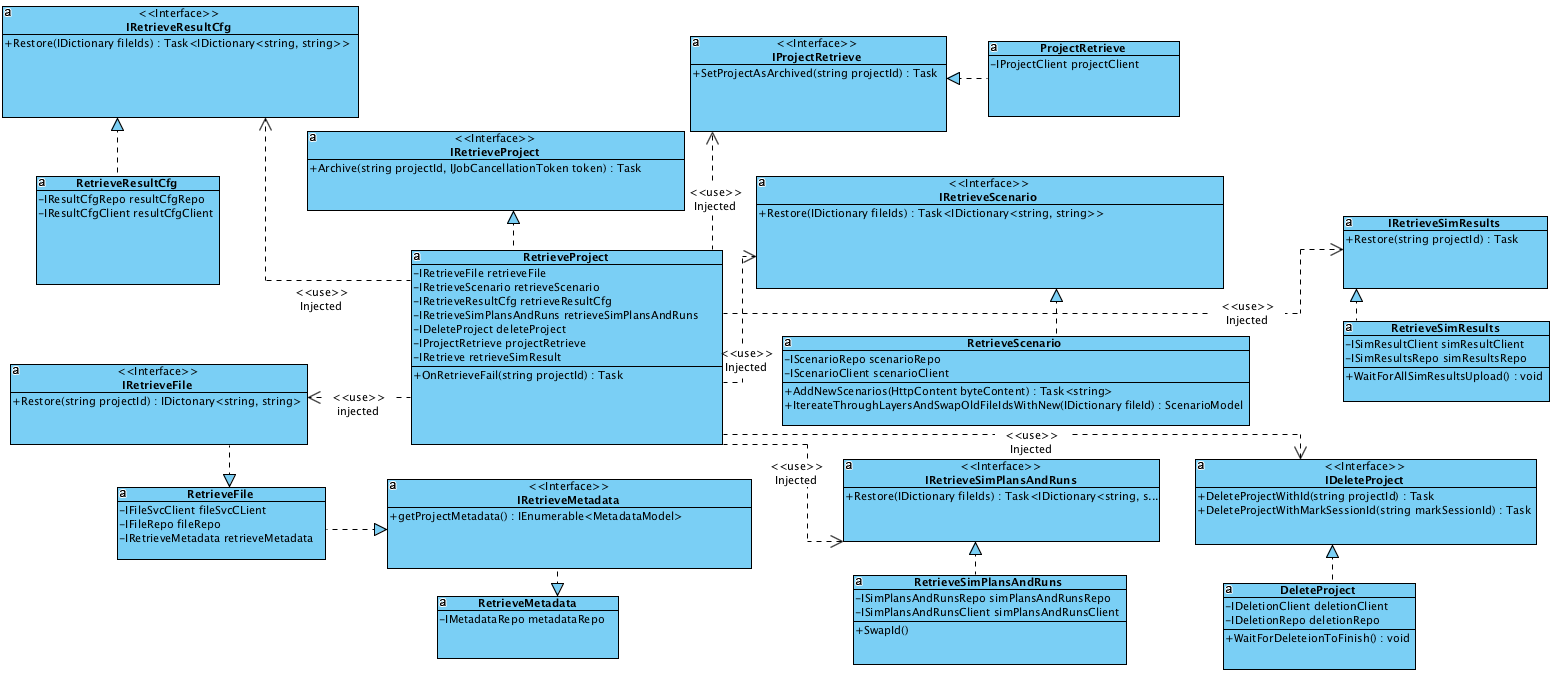
\includegraphics[height=6cm, angle=90, origin=c, width=10.5cm]{grafiken/restoreClass.png}
    \caption{Class Diagram for the Restore process (Top level)}
    \label{fig:restoreClass}
\end{figure}




\newpage
\begin{lstlisting}[caption={Snippet of archived MARS metadata resource}, language=json,firstnumber=1, captionpos=b, label={lst:marsMetadata}]
{
    "DataId":"7cae6055-d7fd-418e-9ba0-bdc2980ffb4c",
    "Title":"KNPGIS.zip",
    "Description":null,
    "ProjectId":"c5deed87-dd03-45c3-a0c4-fdf9f1a307a0",
    "UserId":"af7e045f-edf4-4df5-a9c8-6327186e6ddb",
    "Privacy":"PROJECT_PRIVATE",
    "State":"TO_BE_DELETED"
}
\end{lstlisting}

\begin{lstlisting}[caption={Snippet of the uploaded MARS metadata resource}, language=json,firstnumber=1, captionpos=b, label={lst:marsNewMetadata}]
{
    "DataId":"27765261-8a65-45ab-bdeb-db8b5b7f8f43",
    "Title":"KNPGIS.zip",
    "Description":null,
    "ProjectId":"c5deed87-dd03-45c3-a0c4-fdf9f1a307a0",
    "UserId":"af7e045f-edf4-4df5-a9c8-6327186e6ddb",
    "Privacy":"PROJECT_PRIVATE",
    "State":"TO_BE_DELETED"
}
\end{lstlisting}

\begin{lstlisting}[caption={Snippet of the archived MARS scenario resource}, language=json,firstnumber=1, captionpos=b, label={lst:marsScenario}]
{
    "MetaDataId":"7cae6055-d7fd-418e-9ba0-bdc2980ffb4c",
    "Description":"No description available.",
    "ClearName":"gis_vector_percipitation.zip",
    "AllowedTypes":["SHAPEFILE","GEOJSON"],
    "ParameterMapping":[]
}
\end{lstlisting}

\newpage
\begin{lstlisting}[language={[Sharp]C}, caption={A method in RetrieveScenarios to swap Attributes}, captionpos=b,label={lst:swapCode}]
private async Task<ScenarioModel> ItereateThroughLayersAndSwapOldFileIdsWithNew(IDictionary<string, string> fileIds, ScenarioModel dataScenarioModel)
{
    fileIds.TryGetValue(dataScenarioModel.ModelMetaData, out var newModelId);
    dataScenarioModel.ModelMetaData = newModelId;
    dataScenarioModel.ScenarioId = string.Empty;
    
    foreach (dynamic initializationDescriptionGeoPotentialFieldLayer in dataScenarioModel.InitializationDescription.GeoPotentialFieldLayers)
    {
        fileIds.TryGetValue((string)initializationDescriptionGeoPotentialFieldLayer["MetaDataId"], out var newGeoPotentialId);
        initializationDescriptionGeoPotentialFieldLayer["MetaDataId"] = newGeoPotentialId;
    }
}
\end{lstlisting}